\documentclass[tikz,border=1.35mm]{standalone}

\definecolor{fvmadaptedge}{HTML}{8A7E7E}
\usetikzlibrary{arrows.meta}

\definecolor{externalface}{HTML}{8FB9E8}

% Colored tetrahedral cell figure.
% The cell is drawn as the reference tetrahedron in computational coordinates.
\begin{document}
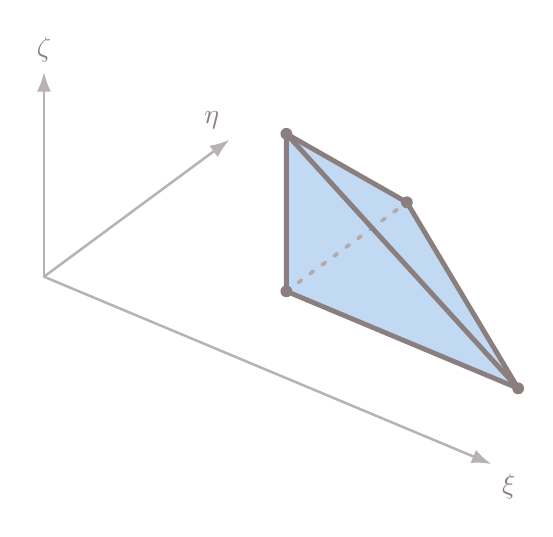
\begin{tikzpicture}[
  x={(20.3mm,-8.5mm)},
  y={(15.3mm,11.3mm)},
  z={(0mm,20mm)},
  line join=round,
  line cap=round,
  outer/.style={draw=fvmadaptedge,line width=0.62mm},
  hidden/.style={draw=fvmadaptedge!65,line width=0.48mm,loosely dotted},
  face/.style={fill=externalface,fill opacity=0.32,draw=none},
  axis/.style={draw=fvmadaptedge!60,line width=0.32mm,-{Latex[length=2.5mm,width=1.8mm]}}
]
  % Reference tetrahedron vertices. The xi direction is stretched to match the
  % prism and hexahedron figures.
  \coordinate (A) at (0,0,0);
  \coordinate (B) at (1.45,0,0);
  \coordinate (C) at (0,1,0);
  \coordinate (D) at (0,0,1);

  % Offset computational-coordinate axes.
  \coordinate (Oaxis) at (-1.20,-0.42,-0.18);
  \draw[axis] (Oaxis) -- (1.60,-0.42,-0.18) node[below right,font=\normalsize,text=fvmadaptedge] {$\xi$};
  \draw[axis] (Oaxis) -- (-1.20,1.12,-0.18) node[above left,font=\normalsize,text=fvmadaptedge] {$\eta$};
  \draw[axis] (Oaxis) -- (-1.20,-0.42,1.12) node[above,font=\normalsize,text=fvmadaptedge] {$\zeta$};

  % Exterior faces share the same translucent shade.
  \path[face] (A) -- (B) -- (C) -- cycle;
  \path[face] (A) -- (B) -- (D) -- cycle;
  \path[face] (A) -- (C) -- (D) -- cycle;
  \path[face] (B) -- (C) -- (D) -- cycle;

  % Hidden-line convention: only the pure eta edge is dotted.
  \draw[hidden] (A) -- (C);

  % Visible exterior wireframe.
  \draw[outer] (A) -- (B);
  \draw[outer] (A) -- (D) -- (B);
  \draw[outer] (B) -- (C) -- (D);

  % Original vertices are #8a7e7e.
  \foreach \p in {A,B,C,D} {
    \fill[fvmadaptedge] (\p) circle[radius=0.75mm];
  }
\end{tikzpicture}
\end{document}
